\chapter{ Etude de l'existant}
\newpage
\textbf{\huge Introduction} \\[1cm]
\textsf{\fontfamily{qtm}\selectfont\scalefont{1.3}
L’objectif de ce deuxième chapitre est la présentation des solutions existantes sur le marché avec une étude comparative et présentation de la solution proposée.
}\\[0.1cm]


\section{\LARGE Les solutions existantes}
\texttt{}\\[0.1cm]
\textsf{\fontfamily{qtm}\selectfont\scalefont{1.3} L'entreprises a des besoins sur mesure. C'est pourqouien revue les solutions similaires à notre solution. Nous allons étudier les points forts ainsi que les points faibles de ces solutions afin de montrer pourquoi nous devrions developper notre propre solution. Voici une présentation de certaines solutions existantes :}
\subsection{\LARGE Azure Devops}
\texttt{}\\[0.1cm]
\textsf{\fontfamily{qtm}\selectfont\scalefont{1.3}Azure DevOps prend en charge une culture collaborative et un ensemble de processus qui rassemblent les développeurs, les responsables de projets et les contributeurs pour développer des logiciels. Elle permet aux organisations de créer et d’améliorer les produits à un rythme plus rapide que possible avec les approches traditionnelles de développement de logiciels.Azure DevOps Services vous donne également accès aux serveurs de génération et de déploiement cloud et aux insights sur les applications. Démarrez gratuitement et créez une organisation. Ensuite, chargez votre code pour partager ou contrôler le code source. Commencez à suivre votre travail à l’aide de Scrum, Kanban ou d’une combinaison de méthodes.(Voir figure 2.1)\cite{9}}
\textsf{\fontfamily{qtm}\selectfont\scalefont{1.3}Elle a des avantages mais aussi des inconvenients:}\\[0.1cm]
\par \noindent \textbf{\Large -Avantage:}
\textsf{\fontfamily{qtm}\selectfont\scalefont{1.3}Azure offre une haute disponibilité,sécurité solide et offre de bonnes options d’évolutivité.}\\[0.1cm]
\par \noindent \textbf{\Large -Inconvenient:}
\textsf{\fontfamily{qtm}\selectfont\scalefont{1.3}oblige à mettre tous vos oeufs dans le même panier et la facilité d’accès peut être problématique pour certaines entreprises.}\\[0.1cm]
\par \noindent \textbf{\Large -Collaboration tools:}
\textsf{\fontfamily{qtm}\selectfont\scalefont{1.3}}
\begin{figure}[H]
    \begin{center}
    
        \fbox{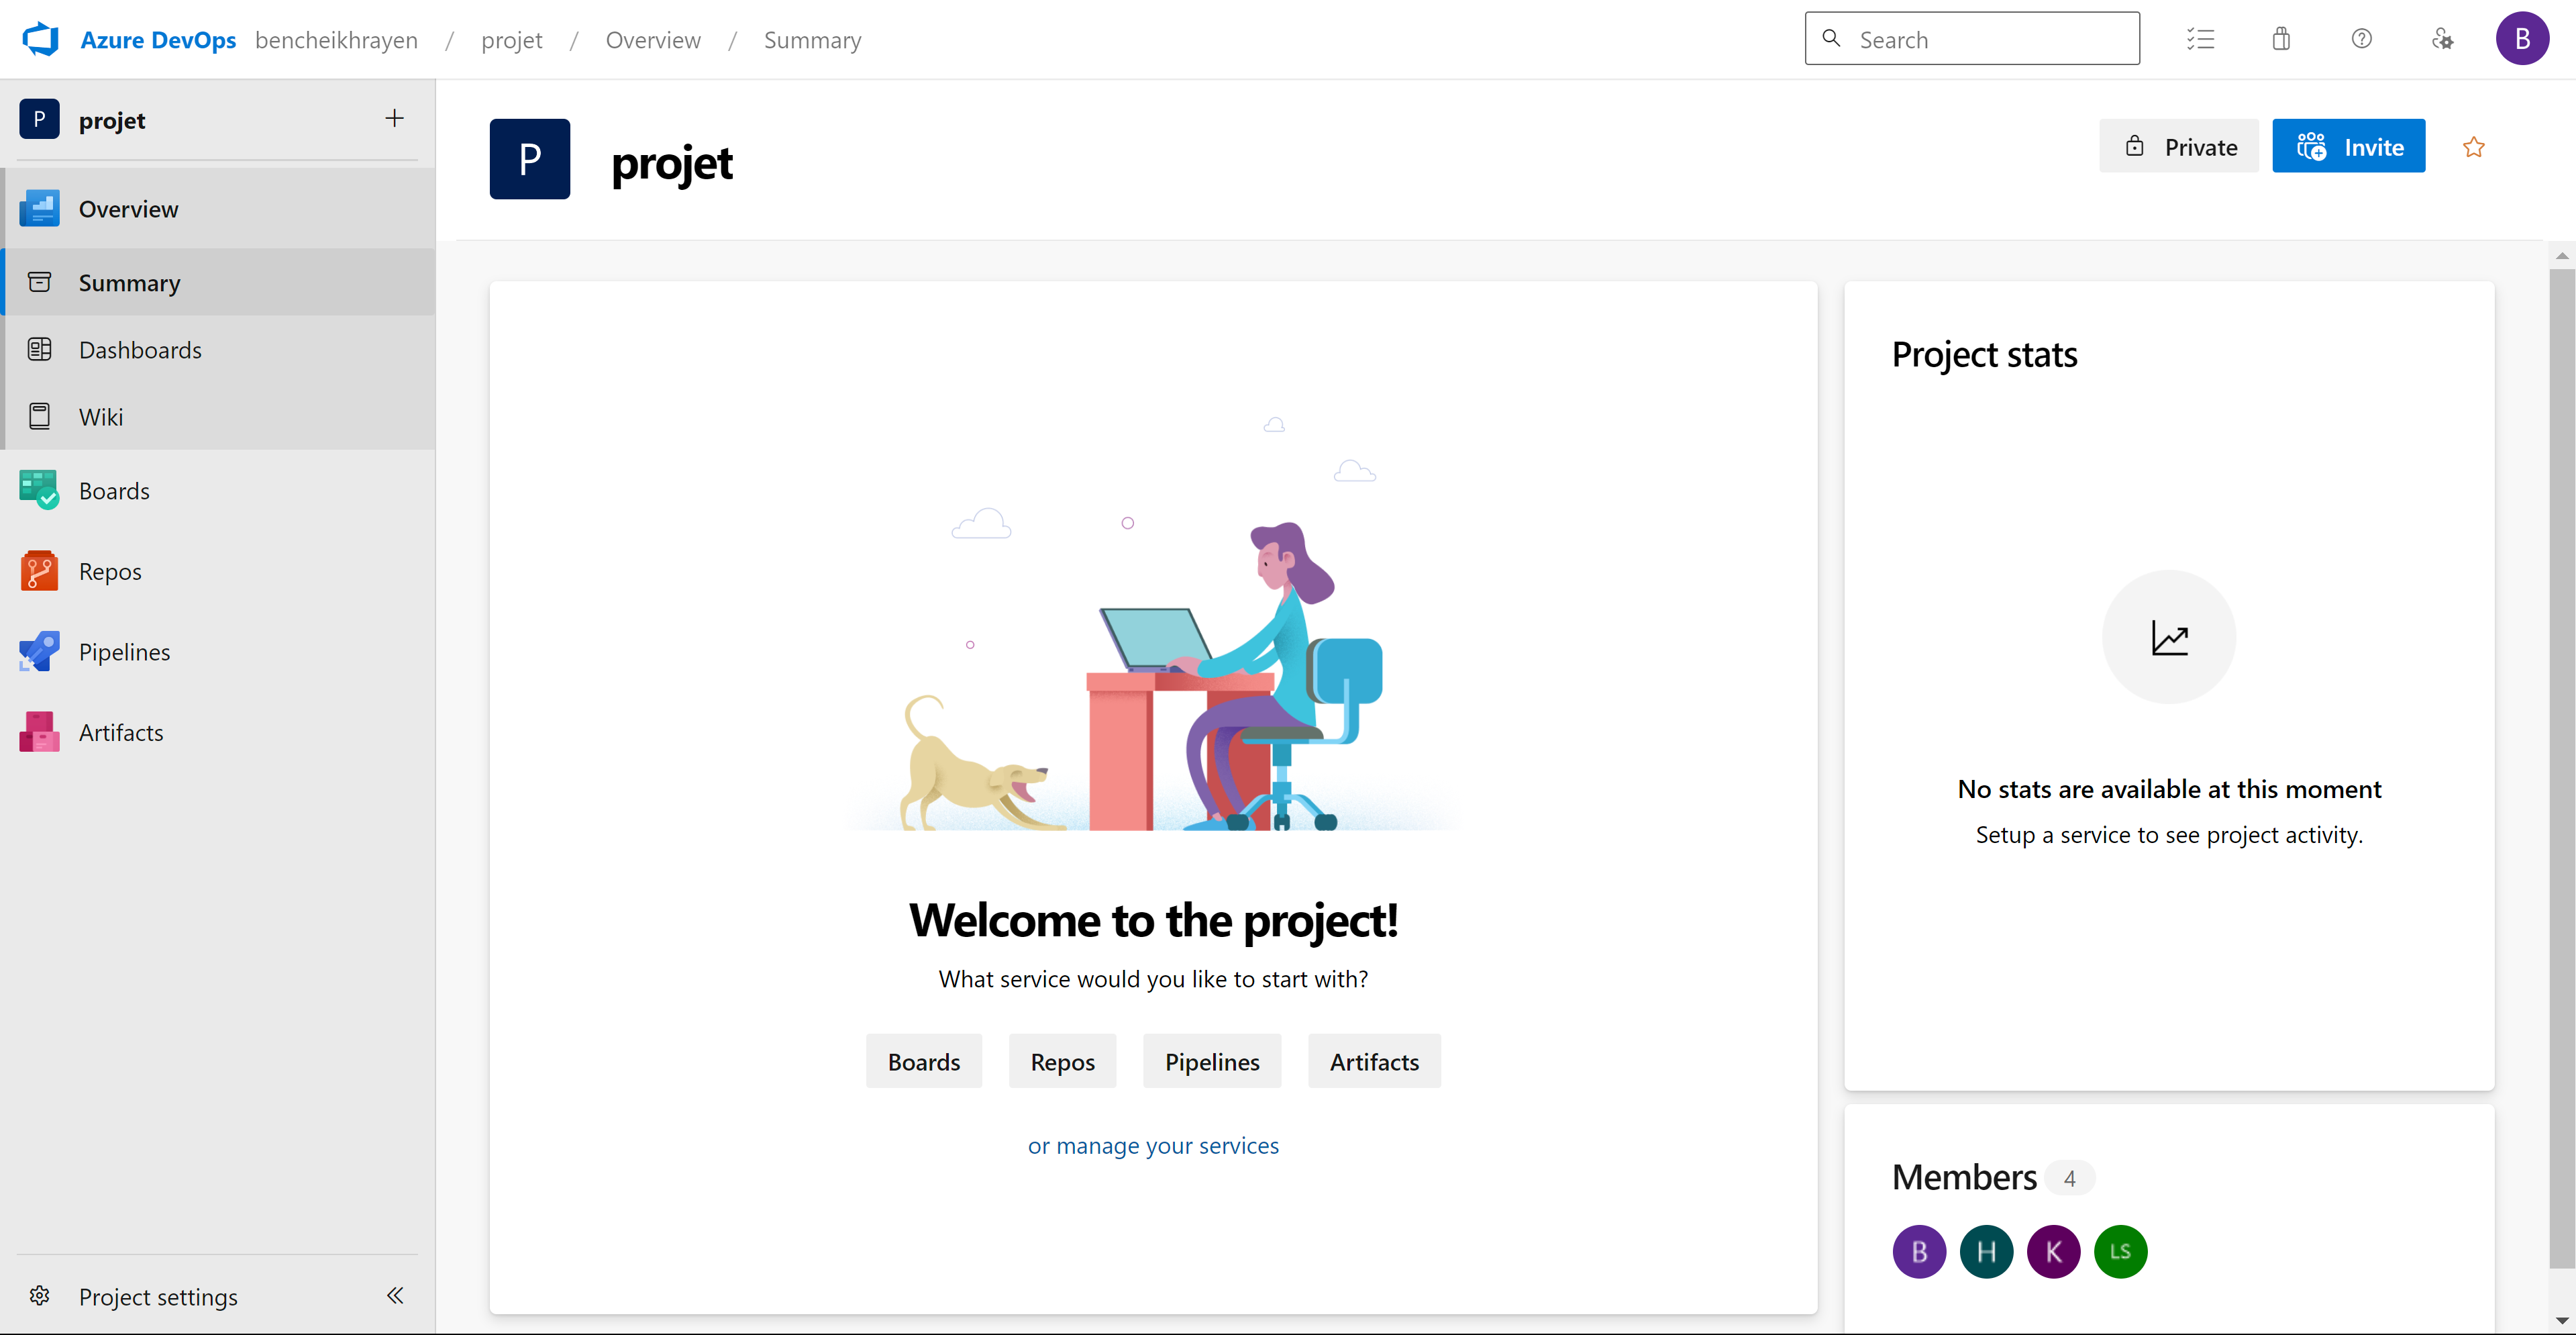
\includegraphics[width=12cm]{azure.png}}

    \end{center}
    
    \caption{Azure DevOps}
\end{figure}

\subsection{\LARGE Amazon Web Service DevOps}
\texttt{}\\[0.1cm]
\textsf{\fontfamily{qtm}\selectfont\scalefont{1.3} AWS fournit un ensemble de services flexibles, conçus pour permettre aux entreprises de créer et livrer des produits avec plus de rapidité et de fiabilité à l'aide d'AWS et des pratiques de DevOps. Ces services simplifient la mise en service et la gestion de l'infrastructure, le déploiement de code d'application, l'automatisation des processus de publication de logiciel et le suivi des performances de l'application et de l'infrastructure(Voir figure 2.2).Cependant, comme toute autre technologie, AWS présente des avantages et des inconvénients: \cite{10}}\\[0.1cm]
\par \noindent \textbf{\Large -Avantage:}
\textsf{\fontfamily{qtm}\selectfont\scalefont{1.3}Aws offre une grande évolutivité pour les entreprises peuvent facilement augmenter ou réduire leurs ressources en fonction de leurs besoins .Aussi , il présente un niveau de fiabilité élevé et il fournit aux entreprises une gamme de services, notamment le stockage, la gestion de bases de données, la puissance de calcul et l’analyse}\\[0.1cm]
\par \noindent \textbf{\Large -Inconvenient:}
\textsf{\fontfamily{qtm}\selectfont\scalefont{1.3}AWS est complexe à mettre en place et à gérer ses ressources. Aussi, les entreprises doivent prendre des mesures pour garantir la protection de leurs données.}
\begin{figure}[H]
  \begin{center}
  
      \fbox{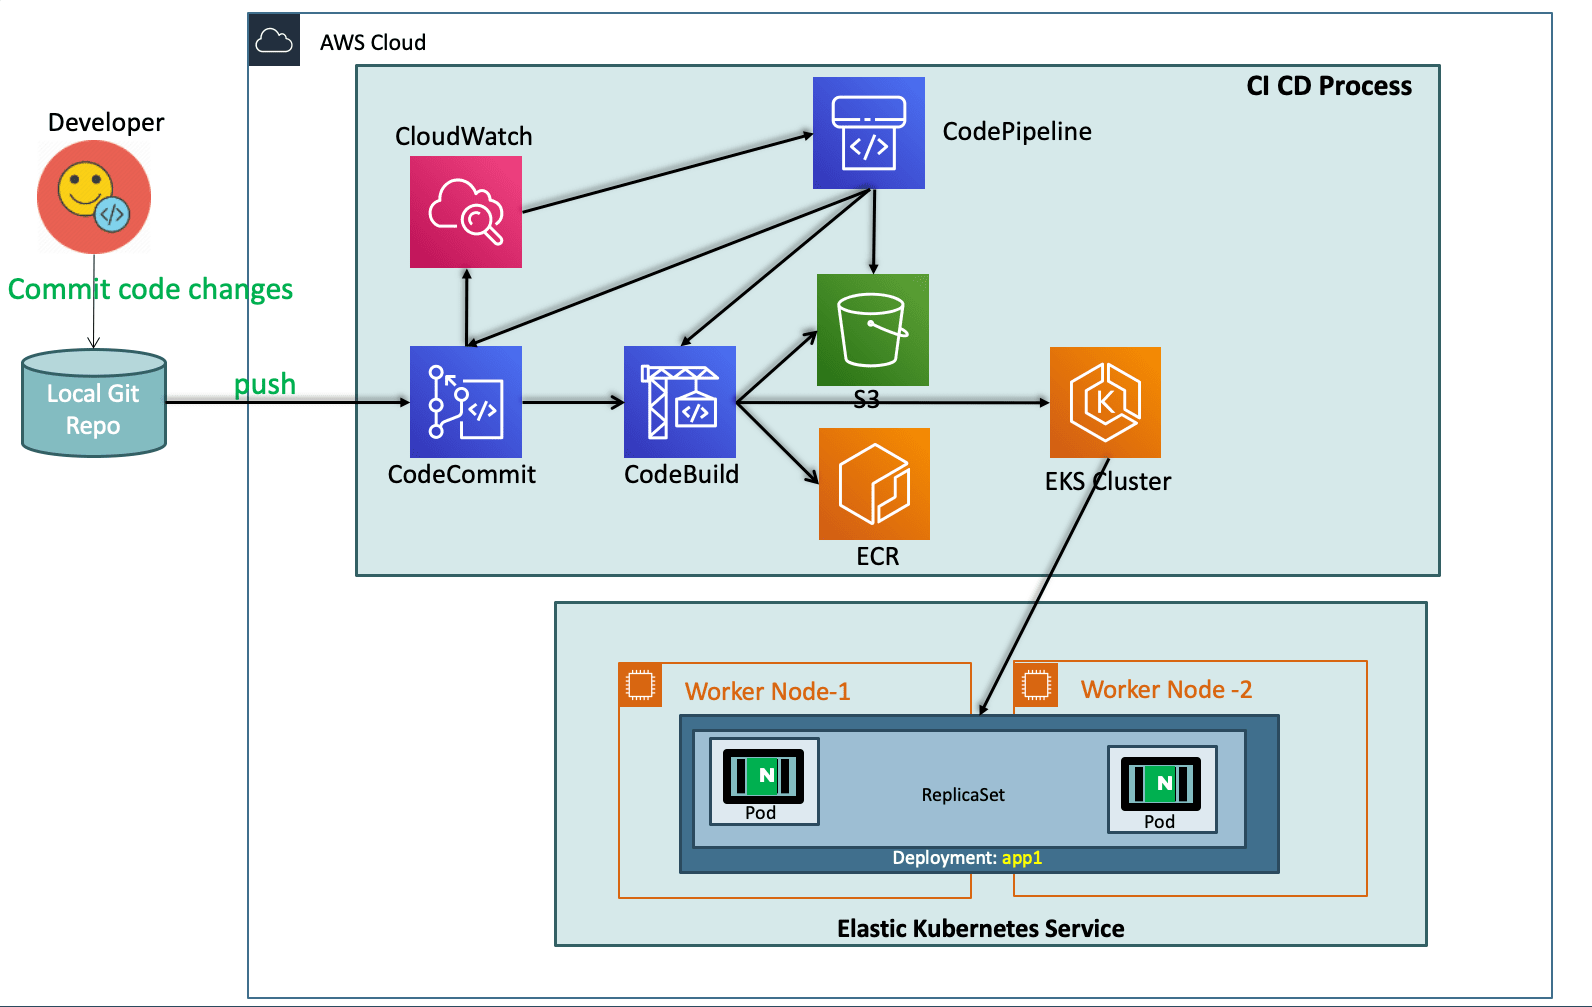
\includegraphics[width=12cm]{aws.png}}

  \end{center}
  
  \caption{Amazon Web Services}
\end{figure}
\subsection{\LARGE Google Cloud Platform DevOps }
\texttt{}\\[0.1cm]
\textsf{\fontfamily{qtm}\selectfont\scalefont{1.3}
Google propose de nombreux services et fonctionnalités visant à aider les ingénieurs DevOps à disposer de tout ce dont ils ont besoin pour respecter les normes de qualité et de sécurité les plus élevées tout en automatisant la majorité du processus.De plus, vous travaillez avec des outils GCP DevOps efficaces qui non seulement augmentent la qualité des applications, mais améliorent également la vitesse du cycle de développement. Ces outils DevOps s’adressent directement aux ingénieurs logiciels car ils permettent une configuration rapide et simple, avec une interface intuitive qui facilite l’utilisation efficace des outils et méthodologies de livraison continue et de déploiement continu (intégration continue/ déploiement continu(CI/CD))(Voir figure 2.3).Ainsi GCP a des points forts et des points faibes:\cite{11}}
\par \noindent \textbf{\Large -Points forts :}
\textsf{\fontfamily{qtm}\selectfont\scalefont{1.3} GCP offre également des services de développement et d’intégration d’applications aussi une bonne Sécurité .}\\[0.1cm]
\par \noindent \textbf{\Large -Points faibles:}
\textsf{\fontfamily{qtm}\selectfont\scalefont{1.3}  certaines intégrations peuvent être plus étroites avec les services et les outils de Google par rapport aux solutions tierces.Aussi ,la  configuration initiale de GCP est complexe en raison de la vaste gamme de services et d'options disponibles.}\\[0.1cm]
\begin{figure}[H]
  \begin{center}
  
      \fbox{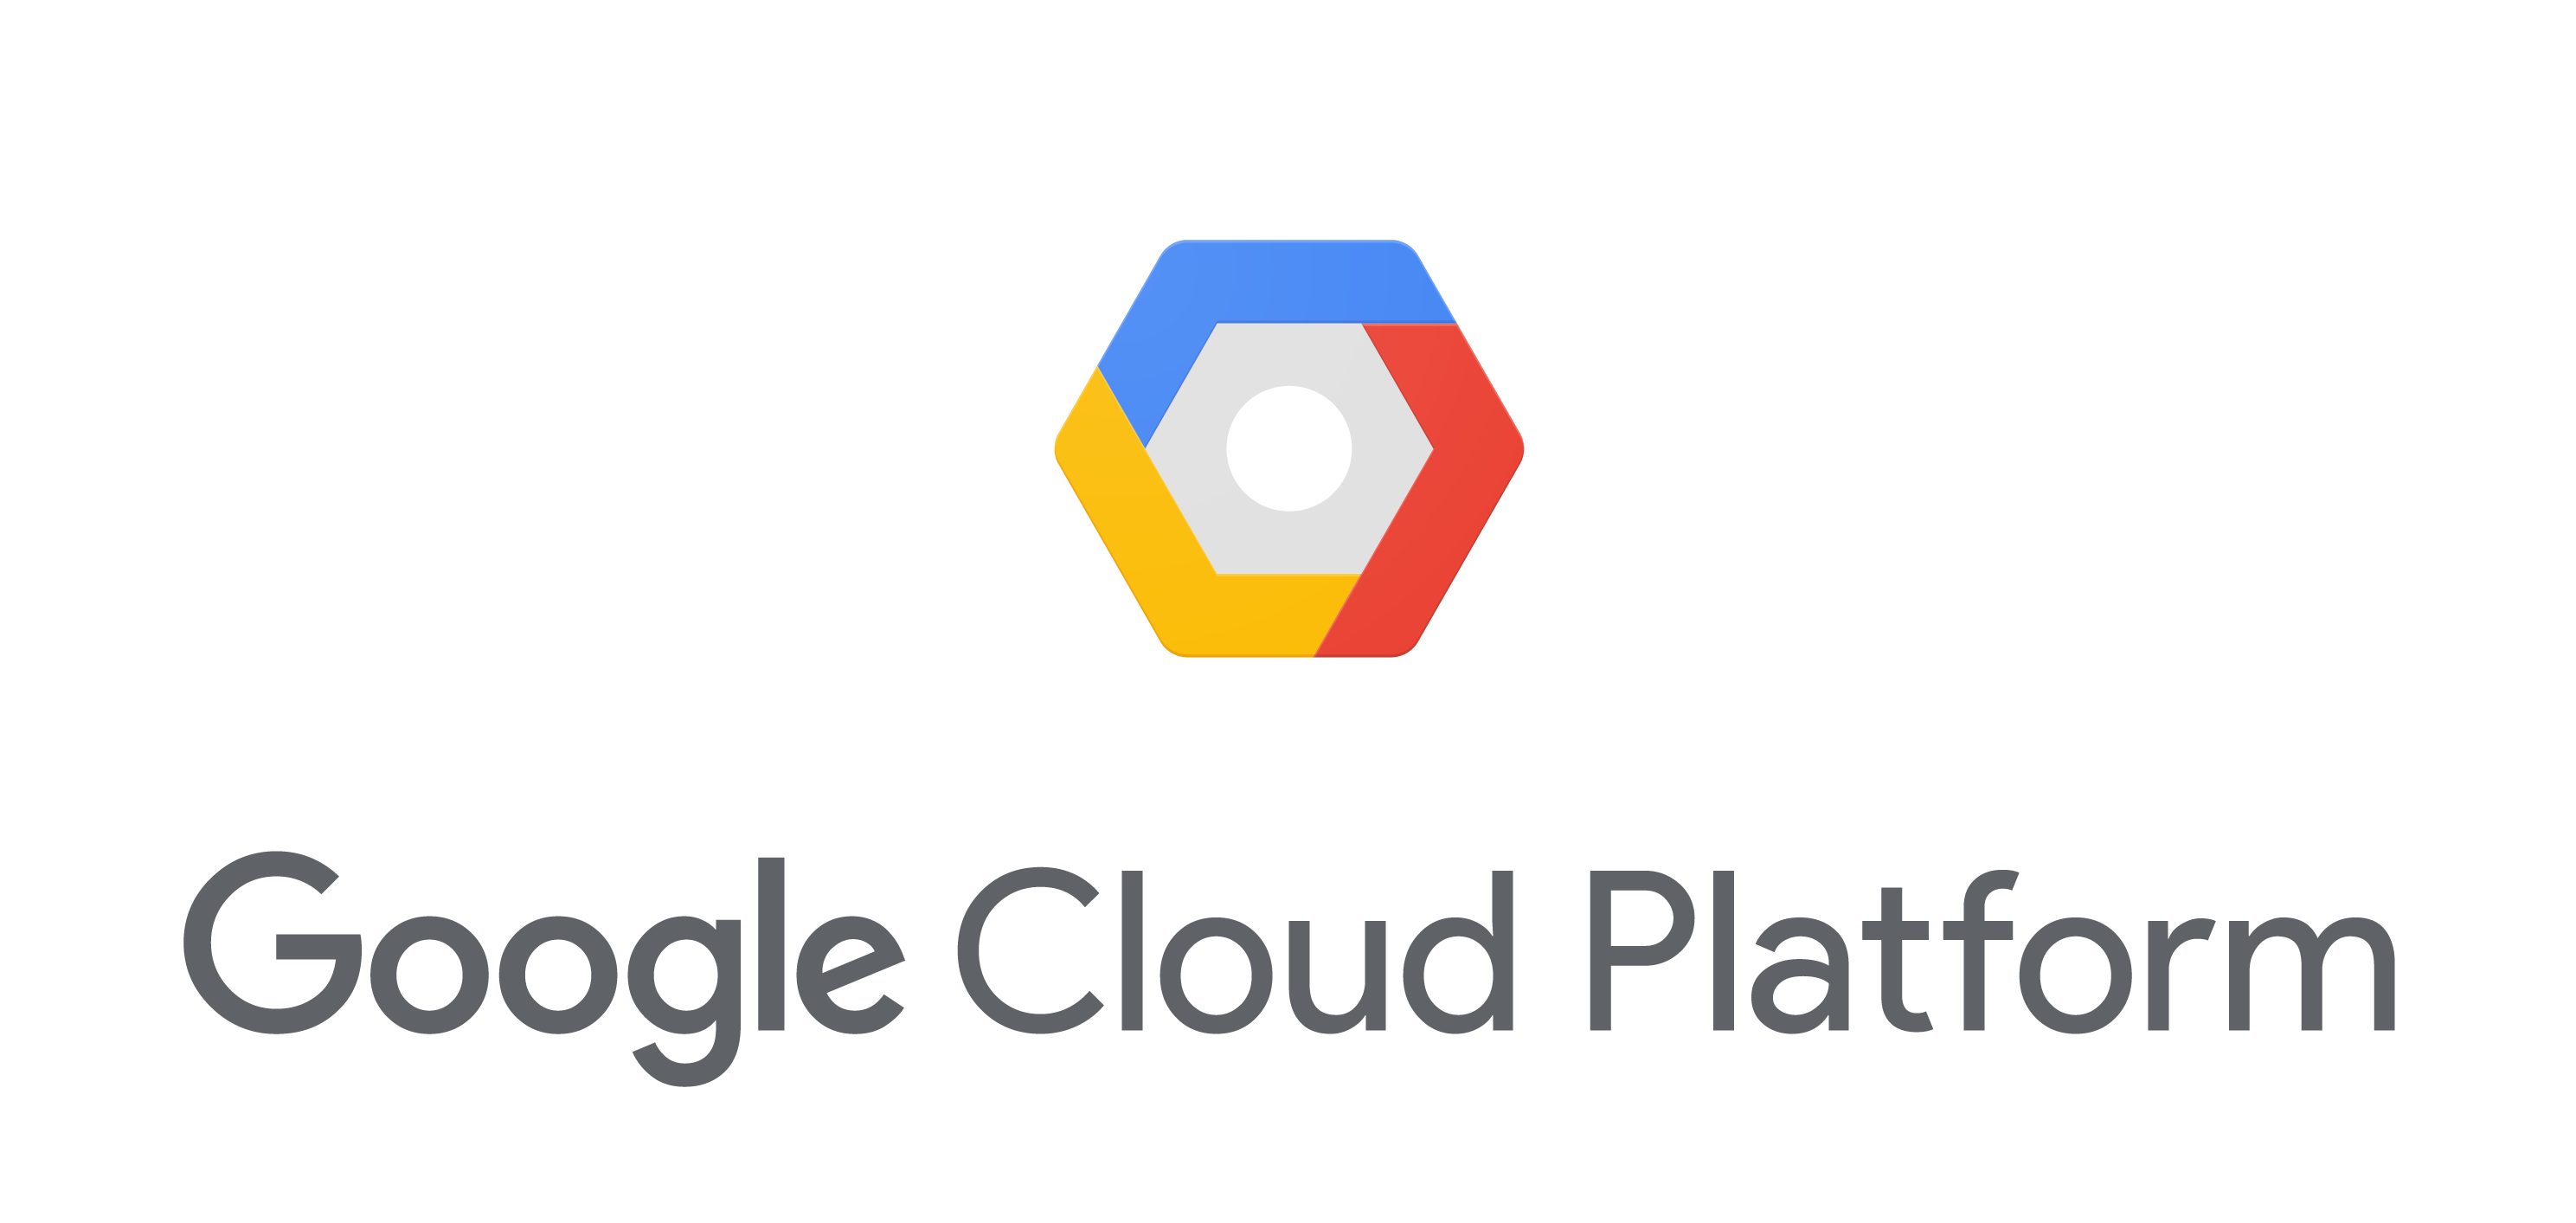
\includegraphics[width=12cm]{gcp.png}}

  \end{center}
  
  \caption{Google Cloud Platform}
\end{figure}
\section{\LARGE Critique des solutions existantes}
\texttt{}\\[0.1cm]
\textsf{\fontfamily{qtm}\selectfont\scalefont{1.3}
Nous allons comparer les solutions présentées ci-dessus selon plusieur qu'on definire par rapport aux besoins de l'entreprise.}\\[0.1cm]
\begin{tabular}{|c|c|c|c|}
\hline
 & Azure Devops & \ Amazon Web Service DevOps & Google Cloud Platform DevOps\\
\hline
C 1 & \textbf{X} &  & \\
\hline
C 2 & & \textbf{X} & \textbf{X} \\
\hline
C 3 & & \textbf{X} &  \\
\hline
C 4 & & & \\
\hline
\end{tabular}
\texttt{}\\[0.1cm]
\textsf{\fontfamily{qtm}\selectfont\scalefont{1.3} En se basant sur le tabeau comparatif ci-dessous,on constate que AWS est plus fiable pour notre sujet mais il n'est pas compatible avec notre projet.}\\[0.1cm]
\par \noindent \textbf{\Large C1 - La confidentialité des données d'application : }\textsf{\fontfamily{qtm}\selectfont\scalefont{1.3} La solution doit privilégier la confidentialité des données puisque certains clients préfèrent leur application exécutée sur le serveur local de la société.} \\[0.1cm]

\noindent \textbf{\Large C2 - Intégration de solutions open source : }\textsf{\fontfamily{qtm}\selectfont\scalefont{1.3} Amazon cloud, azure cloud ou toute autre solution cloud doit intégrer certaines software open source comme services à utiliser dans votre architecture cloud.Bien que les logiciels libres puissent être hautement personnalisables, le niveau de personnalisation fourni par un fournisseur de services peut être restreint. }\\[0.1cm]
\noindent \textbf{\Large C3 - Coût de projet : }\textsf{\fontfamily{qtm}\selectfont\scalefont{1.3}  L'utilisation d'Amazon Cloud ainsi tout autre fournisseur pour  déployer une application dans le Cloud semble peu coûteux au début, mais après que la charge de travail augmente, les coûts aussi augmentent . Il s'agit de trouver une solution qui profite du cloud et des avantages du logiciel libre.}\\[0.1cm]
\noindent \textbf{\Large C4 - Problèmes de compatibilité : }\textsf{\fontfamily{qtm}\selectfont\scalefont{1.3} La personnalisation peut présenter des problèmes de compatibilité, surtout si la personnalisation interagit avec d'autres services ou composants au cours du déploiement. Cela peut entraîner des temps d’arrêt ou d’autres problèmes de performance.}\\[0.5cm]
% \begin{flushleft} 
%   \textsf{\fontfamily{qtm}\selectfont\scalefont{1.8}\hyphenchar\font=-1 -- Voici un tableau récapitulatif de notre analyse de l'existant...\\
%   Légende : \\
% X : la soulution ne conforme pas a la demande de Sujet.\\
% \checkmark : la soulution conforme a la demande de Sujet.\\}
% \end{flushleft}
\textsf{\fontfamily{qtm}\selectfont\scalefont{1.5} --Notons que cette évaluation ne concerne que notre situation, dans d'autres cas les solutions existantes peuvent être utile.  }

%tableau centré à taille variable qui s'ajuste automatiquement suivant la longueur du contenu

% \begin{center}
% \begin{table}[H]  
%   \centering
% \begin{tabular}{|l|l|l|l|l|}
%   \hline
%   Critère/Solution &  GCP DevOps & AWS DevOps & Azure Devops\\
%   \hline
%   La confidentialité des données d'application & & &  \\
%   Intégration de solutions open source &  &  & \\
%   Coût de projet &  &  & \\
%   Problèmes de compatibilité& &  &  \\
%   \hline
% \end{tabular}
% \caption{Tableau comparatif des solutions existantes}
% \end{table}
% \end{center}
\section{\LARGE Solution proposée}
\texttt{}\\[0.1cm]
\textsf{\fontfamily{qtm}\selectfont\scalefont{1.3} Pour rectifier les problèmes auxquels l’équipe devops fait face chaque jour et afin de  préparer un environnement de développement flexible, Mobelite nous a proposé de mettre en place une solution Hybride cloud qui bénéficie à la fois  de certain services de cloud avec un accès privé aux données. En effet, le projet consiste à implémenter la conteneurisation qui nous offrira une virtualisation des ressources de manière légère, flexible et puissante. Le déploiement d’un kubernetes cluster qui est un système de gestion de conteneurs qu'on va utiliser pour optimiser le déploiement des applications avec l’utilisation d’autres produits comme Ansible pour l’optimisation de cette infrastructure. La solution a des objectifs importants pour l’entreprise comme la réduction des coûts de développement et d'exploitation. Le Cycle de développement sera plus court grâce à l'automatisation et le déploiement rapide des nouveaux environnements.Aussi, la solution garantira la supervision totale et continue de la plateforme, et la haute disponibilité du système.}\\[0.1cm]
\section{\LARGE    Conclusion}
\texttt{}\\[0.3cm]
\textsf{\fontfamily{qtm}\selectfont\scalefont{1.3} Dans ce chapitre, nous avons réalisé une étude de quelques solutions existantes, puis nous avons réalisé une comparaaison de l'existant pour connaître les solutions compatibles avec notre sujet. Après cela, nous avons présente la solution proposée par mobelite.
}